\documentclass[9pt,onecolumn,twoside,]{pinp}

%% Some pieces required from the pandoc template
\providecommand{\tightlist}{%
  \setlength{\itemsep}{0pt}\setlength{\parskip}{0pt}}

% Use the lineno option to display guide line numbers if required.
% Note that the use of elements such as single-column equations
% may affect the guide line number alignment.

\usepackage[T1]{fontenc}
\usepackage[utf8]{inputenc}
\usepackage{subfigure}

% pinp change: the geometry package layout settings need to be set here, not in pinp.cls
\geometry{layoutsize={0.95588\paperwidth,0.98864\paperheight},%
  layouthoffset=0.02206\paperwidth, layoutvoffset=0.00568\paperheight}

\definecolor{pinpblue}{HTML}{af1d18}  % imagecolorpicker on blue for new R logo
\definecolor{pnasbluetext}{RGB}{101,0,0} %



\title{Parcial 3}

\author[a]{David Londoño Lopera}
\author[b]{Cristian Camilo Gañan}

  \affil[a]{CC: 1035440879, Departamento de ciencias forestales, Univeridad Nacional de Colombia,
Medellín}

  \affil[b]{CC: 1059710617, Departamento de ciencias forestales, Univeridad Nacional de Colombia,
Medellín}

\setcounter{secnumdepth}{0}

% Please give the surname of the lead author for the running footer
\leadauthor{Gañan-Londoño}

\doifooter{Depertamento de ciencias forestales}

\pinpfootercontents{Medición forestal}
% Keywords are not mandatory, but authors are strongly encouraged to provide them. If provided, please include two to five keywords, separated by the pipe symbol, e.g:



% initially we use doi so keep for backwards compatibility
% new name is doi_footer


\begin{document}

% Optional adjustment to line up main text (after abstract) of first page with line numbers, when using both lineno and twocolumn options.
% You should only change this length when you've finalised the article contents.
\verticaladjustment{-2pt}

\maketitle
\thispagestyle{firststyle}
\ifthenelse{\boolean{shortarticle}}{\ifthenelse{\boolean{singlecolumn}}}{}

% If your first paragraph (i.e. with the \dropcap) contains a list environment (quote, quotation, theorem, definition, enumerate, itemize...), the line after the list may have some extra indentation. If this is the case, add \parshape=0 to the end of the list environment.


\hypertarget{calculo-del-volumen-usando-la-ecuaciuxf3n-de-smalian}{%
\section{1) Calculo del volumen usando la ecuación de
Smalian}\label{calculo-del-volumen-usando-la-ecuaciuxf3n-de-smalian}}

Para el cálculo de volumen, se utilizó el volumen de fustes estimado por
Smalian, el cual para una troza el volumen es igual a:
\[V_t= (AB_1 \ + \ AB_2)*L\] Esto se puede despejar como:
\[\frac{\pi}{8} \ * \ L(d_1^2*d_2^2)\] Ahora para un fuste completo
sería: \[V_t= L*[\sum_{i=1}^{n}{d_i^2+d_{i+1}^2}] * \frac{\pi}{8}\] Como
se tenían longitudes (\(L\)) variables entonces la fórmula final queda
como:
\[V_t= [\sum_{i=1}^{n}{(d_i^2+d_{i+1}^2)* (L_{i+1}-L_{i}})] * \frac{\pi}{8}\]

\hypertarget{seleccuxf3n-de-muestras-aleatorias-para-construcciuxf3n-de-modelos}{%
\section{2) Seleccón de muestras aleatorias para construcción de
modelos}\label{seleccuxf3n-de-muestras-aleatorias-para-construcciuxf3n-de-modelos}}

Al utilizar la función \texttt{sample()} entre \(1\) y \(100\), dió como
resultado \(32\), este número se utilizó para \texttt{set.seed()} con el
fin de que sacara los mismos valores al seleccionar el \(70 \%\) de los
datos y su respectivo archivo de validación.

\hypertarget{modelos-de-volumen}{%
\subsection{3) Modelos de volumen}\label{modelos-de-volumen}}

En la \textbf{Table 1} se tiene la comparación de los modelos de volumen
a saber:

\begin{enumerate}
\def\labelenumi{\arabic{enumi})}
\tightlist
\item
  \[V \ = \ b_0 + b_1*D+b_2*D^2+b_3*H+b_4*H^2\]
\item
  \[V \ = \ b_0+b_1*(D^2*H)\]
\item
  \[V \ = \ b_0 * D^{b_1}*H^{b_2}\]
\item
  \[V \ = \ b_0*(D^2*H)^{b_1}\]
\end{enumerate}

Al comparar los modelos lineales, aunque es mejor el segundo al tener un
RSE menor que el primero, se descartan ambos modelos debido a que
ninguno es normal y ambos tienen problemas de heterocedasticidad, su
gráfico de residuales tiene forma de ``V'' acostada lo cual sugiere
errores con distribución exponencial o logarítmica . Con relación a los
2 modelos exponenciales se escoge el cuarto como el mejor, pues tiene un
AIC y un RSE menores que los del tercero, en la \textbf{Fig.1} se
muestra la gráfica del modelo, se muestra el buen ajuste que
gráficamente se presenta, este refleja como el \(volumen\) aumenta a
medida que el \(DAP\) y la \(altura\) también lo hacen. En la
\textbf{Table 2} se presenta la validación del modelo, es evidente como
el modelo 4 es el mejor y por mucho pues la media y desviación estándar
son mucho menores que las del modelo 3, señalando así errores bajos con
dispersiones entre el valor real y el estimado.

\begin{table*}[h!]

\caption{\label{tab:unnamed-chunk-9}Comparación de modelos}
\centering
\begin{tabular}[t]{l|r|l|r|r|r|r}
\hline
Modelo & Fc & valor.p & Shapiro & R.squared & AIC & RSE\\
\hline
V= 7.61e-01+(-1.30e-02*D+
               (8.69e-04*D\textasciicircum{}2)+(-1.09e-01*H)+
               (4.19e-03*H\textasciicircum{}2) & 395.9044 & *** & 0.0000 & 0.9577 & -53.01262 & 0.1623729\\
\hline
V= 2.44e-02+3.72e-05*(D\textasciicircum{}2*H) & 2336.9484 & *** & 0.0000 & 0.9697 & -84.11330 & 0.1345016\\
\hline
V= 6.40e-04*D\textasciicircum{}6.15*H\textasciicircum{}3.28 & 2444.2628 & *** & 0.8866 & 0.9855 & -74.91925 & 14.3482000\\
\hline
V= 5.88e-05*(D\textasciicircum{}2*H)\textasciicircum{}2.61 & 4304.9706 & *** & 0.3458 & 0.9833 & -66.51527 & 0.1320000\\
\hline
\end{tabular}
\end{table*}

\begin{figure}

{\centering 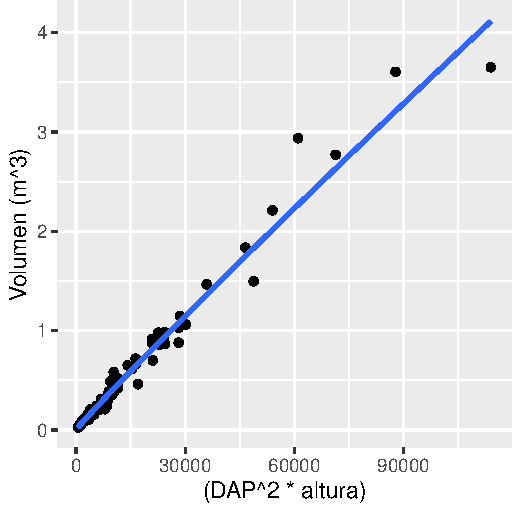
\includegraphics{David_Londono_Lopera_Cristian_Ganan_parcial3_files/figure-latex/unnamed-chunk-10-1} 

}

\caption{Modelo de Volumen}\label{fig:unnamed-chunk-10}
\end{figure}

\begin{table}

\caption{\label{tab:unnamed-chunk-11}Validación de modelos volumen}
\centering
\begin{tabular}[t]{r|r|r|r}
\hline
Media3 & sd3 & Media4 & sd4\\
\hline
-1520.335 & 185.554 & -3.03686 & 14.20831\\
\hline
\end{tabular}
\end{table}

\hypertarget{calculo-de-biomasa}{%
\section{4) Calculo de biomasa}\label{calculo-de-biomasa}}

Para calcular la biomasa, primero se halló el contenido de humedad de
las rodajas de fuste, ramas y hojas por medio de la siguiente fórmula:
\[CH \ = \ \frac{Peso \ verde-Peso \ seco}{Peso \ verde}\] Después se
determinó la biomasa aérea de cada uno de los componentes así:
\[BA \ = \ P_{verde \ total}* (1-CH)\]

Cabe aclarar que para la biomasa del fuste completo, se juntaron las
biomasas de cada troza. Finalmente se sumaron las biomasas obtenidas del
fuste, ramas y hojas para así tener la biomasa total en \(kg\).

\hypertarget{modelos-de-biomasa-uxe1erea}{%
\section{5) Modelos de biomasa
áerea}\label{modelos-de-biomasa-uxe1erea}}

Para poder aplicar los modelos de Biomasa, se calculó la densidad de la
madera (\(WD\)), ya que algunos modelos la requerían:
\[\rho \ = \  \frac{Peso \ seco \ rodaja (Kg)}{ V(m^3)}\]
\[V \ = \ area \ rodaja (m^2) * Espesor \ rodaja (m)\] Después de hallar la
biomasa total y la densidad de madera se seleccionaron 80\% de los datos
para ajustar el modelo, de tal forma que como el total eran \(31\)
entonces: \[31*0.80= 25 \ datos \ para \ el \ modelo\] Los modelos
ajustados son los siguientes:

\begin{enumerate}
\def\labelenumi{\alph{enumi})}
\tightlist
\item
  \[BA \ = \ b_0 + b_1*D+b_2*H\]
\item
  \[BA \ = \ b_0+b_1(D^2*H)\]
\item
  \[BA \ = \ b_0*D^{b_1}*H^{b_2}\]
\item
  \[BA \ = \ b_0*D^{b_1}*H^{b_2}*WD^{b_3}\]
\item
  \[BA \ = \ b_0*(D^2*WD)^{b_1}\]
\item
  \[BA \ = \ b_0*(D^2*H)^{b_1}\]
\item
  \[BA \ = \ b_0*(D^2*H*WD)^{b_1}\]
\end{enumerate}


\begin{figure}[!h]

{\centering 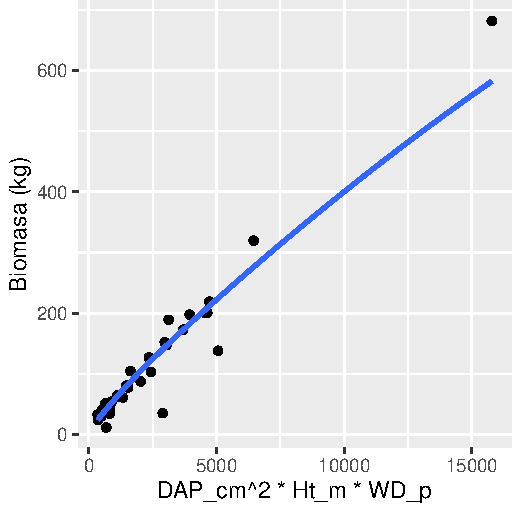
\includegraphics{David_Londono_Lopera_Cristian_Ganan_parcial3_files/figure-latex/unnamed-chunk-23-1} 

}

\caption{Modelo de Biomasa}\label{fig:unnamed-chunk-23}
\end{figure}

\begin{table*}[h]

\caption{\label{tab:unnamed-chunk-24}Modelos de Biomasa}
\centering
\begin{tabular}[t]{l|r|l|r|r|r|r}
\hline
Modelo & Fc & valor.p & Shapiro & R.squared & AIC & RSE\\
\hline
BA= -207.20+18.34*D+(-0.3342*H) & 39.6762 & *** & 0.0201 & 0.7829 & 286.14189 & 67.20959\\
\hline
BA= 3.75+0.025*(D\textasciicircum{}2*H) & 308.0868 & *** & 0.0032 & 0.9305 & 255.65875 & 37.18581\\
\hline
BA= 0.12*D\textasciicircum{}15.31*H\textasciicircum{}0.62 & 55.6392 & *** & 0.0073 & 0.8349 & 28.44571 & 52.93970\\
\hline
BA= 0.16*D\textasciicircum{}11.33*H\textasciicircum{}0.93*WD\textasciicircum{}2.16 & 51.5368 & *** & 0.0000 & 0.8513 & 29.23174 & 41.89810\\
\hline
BA= 0.23*(D\textasciicircum{}2*WD)\textasciicircum{}3.23 & 161.7459 & *** & 0.0000 & 0.8480 & 25.92556 & 40.08310\\
\hline
BA= 0.10*(D\textasciicircum{}2*H)\textasciicircum{}2.32 & 111.2088 & *** & 0.0000 & 0.7932 & 35.46763 & 42.46070\\
\hline
BA= 0.18*(D\textasciicircum{}2*H*WD)\textasciicircum{}2.31 & 91.9029 & *** & 0.0000 & 0.7998 & 31.26584 & 38.53990\\
\hline
\end{tabular}
\end{table*}

En la \textbf{Table 3} se muestran los modelos ajustados para la
biomasa, los lineales se descartan pues no cumplen con los supuestos
para este tipo de regresión, respecto a los exponenciales, el modelo
\textbf{e} tiene el menor AIC entre todos los modelos exponenciales, sin
embargo, al comparar el \(RSE\), es evidente que el mejor modelo es el
\textbf{g}, pues es el que presenta el menor valor,teniendo en cuenta
que el \(AIC\) es un estimador del error de predicción fuera de la
muestra y el \(RSE\) el error de los residuales, se adopta como mejor
modelo al \textbf{g} pues tiene un error pequeño y un capacidad de
predicción aceptable. En la \textbf{Table 4} se presenta la validación
del modelo, a pesar de que el modelo \textbf{e} tiene una media menor
que del \textbf{g}, este presenta una desviación muy alta en comparación
con el \textbf{g} esto indica que el modelo \textbf{e} tiende a
subestimar mucho pues su valor predicho se aleja en buena medida del
valor real.

\begin{table}[h]

\caption{\label{tab:unnamed-chunk-25}Validación de modelo Biomasa}
\centering
\begin{tabular}[t]{r|r|r|r}
\hline
Media\_g & sd\_g & Media\_e & sd\_e\\
\hline
-11.85311 & 26.66373 & -22.19342 & 54.67461\\
\hline
\end{tabular}
\end{table}

\hypertarget{estimacuxf3n-de-volumen-y-biomasa-en-cinco-localidades}{%
\subsection{6) Estimacón de volumen y biomasa en cinco
localidades}\label{estimacuxf3n-de-volumen-y-biomasa-en-cinco-localidades}}

Se estimó el volumen y la biomasa de las parcelas, usando los modelos
seleccionados anteriormente, en las siguientes localidades: Anorí,
Caicedo, Maceo, Porce y Ventanas. Para hallar el contenido de carbono
almacenado se multiplicó la biomasa por \(0.5\), el cual es el factor de
conversión del \(IPCC\). En la \textbf{Table 5} y \textbf{Table 6} se
muestra la media y desviación estándar del volumen y del contenido de
carbono, respectivamente, con relación al volumen se puede decir que es
un valor promedio aceptable pues, según el modelo de escogido
\textbf{Fig.1} la tasa de cambio del volumen respecto al \(DAP\) y
\(altura\) tiende a ser constante, por ende, se presenta una relación
directamente proporcional entre las variables; la misma situación ocurre
con el contenido de carbono solo que en este caso, el modelo de biomasa
\textbf{Fig.2} sugiere una curva un poco convexa que podría
interpretarse como una acumulación de biomasa más rápida en estadios
jóvenes de los bosques, con una leve caída al final pero sin dejar de
aumentar a medida que el \(DAP\) y la \(altura\) lo hacen, este
comportamiento hace que el valor del contenido de carbono tienda a ser
constante.

\begin{table}

\caption{\label{tab:unnamed-chunk-29}Volumen del inventario}
\centering
\begin{tabular}[t]{r|r}
\hline
Media & Desviacion\\
\hline
77.58832 & 103.0507\\
\hline
\end{tabular}
\end{table}

\begin{table}

\caption{\label{tab:unnamed-chunk-30}Contenido de Carbono del iventario}
\centering
\begin{tabular}[t]{r|r}
\hline
media contenido de C & Sd contenido de C\\
\hline
2.175178 & 2.451563\\
\hline
\end{tabular}
\end{table}

\hypertarget{comparaciuxf3n-entre-localidades}{%
\section{7) Comparación entre
localidades}\label{comparaciuxf3n-entre-localidades}}

Para el volumen hay diferencias significativas entre Anorí y Maceo
(\textbf{Fig.3 (a)}), las demás localidades resultan ser iguales, es
interesante mirar los puntos extremos que se presentan, esto hace que
las pruebas de tendencia central puedan verse perturbadas, causando
quizás que en teoría los volúmenes sean iguales pero se diferencien por
valores extremos; puede notarse también una relación dependiente entre
el volumen y la biomasa, pues las mismas localidades que resultaron
diferentes en cuanto a volumen también son diferentes en Biomasa
(\textbf{Fig.3 (b)}), esto quizás se deba a que los muestreos hechos
tuvieron ejemplares con grandes edades ,lo que los hace diferentes en
cuanto al \(DAP\) y \(altura\) del resto, es común encontrar este tipo
de comportamiento en lugares que han sido intervenidos y posteriormente
abandonados.

\begin{figure}[htbp]
\centering
\subfigure[Comparación de volumen por Localidad]{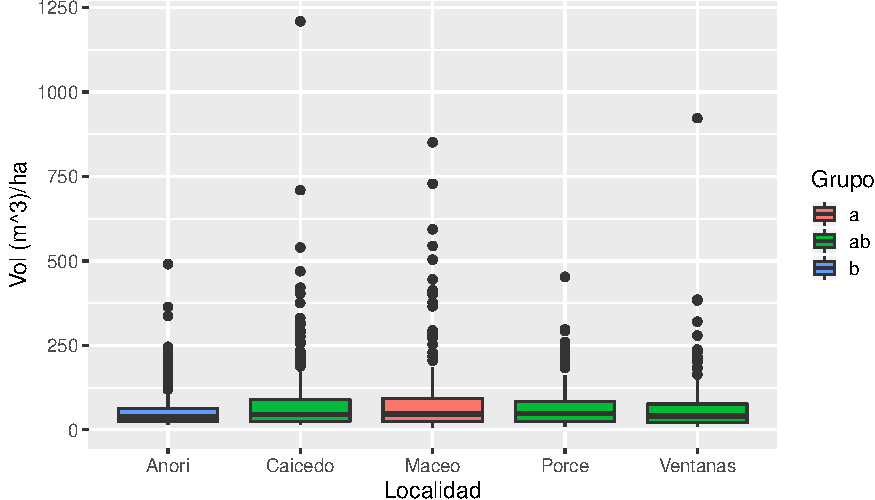
\includegraphics[width=80mm]{David_Londono_Lopera_Cristian_Ganan_parcial3_files/figure-latex/unnamed-chunk-31-1}}
\subfigure[Comparación de Biomasa por Localidad]{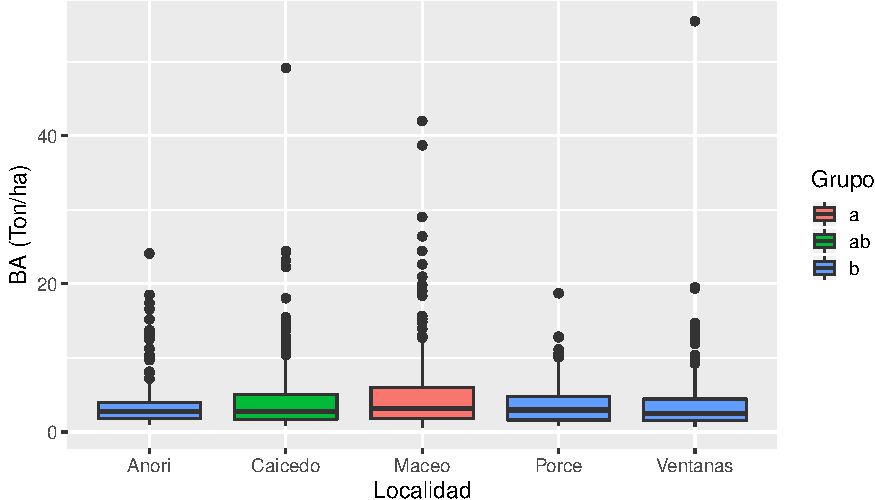
\includegraphics[width=80mm]{David_Londono_Lopera_Cristian_Ganan_parcial3_files/figure-latex/unnamed-chunk-32-1}}
\caption{Comparación por localidad} \label{fig:lego}
\end{figure}

%\showmatmethods

\pnasbreak 




\end{document}

